% ----------------------------------------------------------------
%% Thesis.tex -- MAIN FILE (the one that you compile with LaTeX)
%% ---------------------------------------------------------------- 

% Set up the document
\documentclass[a4paper, 11pt, oneside]{Thesis}  % Use the "Thesis" style, based on the ECS Thesis style by Steve Gunn
%\graphicspath{Figures/}  % Location of the graphics files (set up for graphics to be in PDF format)
\usepackage{fancyhdr}
% Include any extra LaTeX packages required
\usepackage[square, numbers, comma, sort&compress]{natbib}  % Use the "Natbib" style for the references in the Bibliography
\usepackage{verbatim}  % Needed for the "comment" environment to make LaTeX comments
\usepackage{vector}  % Allows "\bvec{}" and "\buvec{}" for "blackboard" style bold vectors in maths
\usepackage{graphicx} 
\hypersetup{urlcolor=blue, colorlinks=true}  % Colours hyperlinks in blue, but this can be distracting if there are many links.
%
\pagestyle{fancy}
\fancyhf{}  % Alle Kopfzeilen löschen
%% ----------------------------------------------------------------
\begin{document}
\begin{titlepage}

\newcommand{\HRule}{\rule{\linewidth}{0.5mm}} % Defines a new command for the horizontal lines, change thickness here

\center % Center everything on the page
 %----------------------------------------------------------------------------------------
%	LOGO SECTION
%----------------------------------------------------------------------------------------
\begin{minipage}{0.4\textwidth}
\begin{flushleft} \large
\includegraphics[width=5cm, height=1.2cm]{Pictures/UST.jpg}
\end{flushleft}
\end{minipage}

\begin{minipage}{0.4\textwidth}
\begin{flushright} \large
\includegraphics[width=5cm, height=1.2cm]{Pictures/ILH.jpg}
\end{flushright}
\end{minipage}\\[2cm]
 % Include a department/university logo - this will require the graphicx package
%----------------------------------------------------------------------------------------
%	HEADING SECTIONS
%----------------------------------------------------------------------------------------

\textsc{\LARGE \bfseries Fachpraktikum (Bachelor)}\\[0.2cm] % Name of your university/college
\textsc{\LARGE 6G Hardwarelabor - Design und Implementierung eines HF Transceivers}\\[0.2cm] 
%\textsc{\LARGE Design}\\[0.5cm] 
%\textsc{\Large ILH}\\[0.5cm] % Major heading such as course name
%\textsc{\large PuL-Analog Microwave Frontend Design}\\[0.5cm] % Minor heading such as course title

%----------------------------------------------------------------------------------------
%	TITLE SECTION
%----------------------------------------------------------------------------------------

\HRule \\[0.4cm]
{ \huge \bfseries Versuch 1: Drahtlose Übertragungen und Link-Budget}\\[0.4cm] % Title of your document
\HRule \\[1.5cm]
 
%----------------------------------------------------------------------------------------
%	AUTHOR SECTION
%----------------------------------------------------------------------------------------
\textbf{Protokollanten}\\
{\large\ Lukas Müller}\\[0.5cm]
{\large\ Erik Zimmerman}\\[0.2cm]
{\large\ Farhad Valizada}\\[0.2cm]

\textbf{Betreuer}\\
{\large\ Simon Haussmann}\\[0.2cm]



%----------------------------------------------------------------------------------------
%	DATE SECTION
%----------------------------------------------------------------------------------------
\textbf{Eingereicht}\\
{\large \today} % Date, change the \today to a set date if you want to be precise

 
%----------------------------------------------------------------------------------------

\vfill % Fill the rest of the page with whitespace

\end{titlepage}


%\vfill\vfill\vfill\vfill\vfill\vfill\null
\clearpage  % Funny Quote page ended, start a new page
%% ----------------------------------------------------------------

% The Abstract Page


%% ----------------------------------------------------------------

\setstretch{1.3}  % Reset the line-spacing to 1.3 for body text (if it has changed)

% The Acknowledgements page, for thanking everyone
%\acknowledgements{
%\addtocontents{toc}{\vspace{1em}}  % Add a gap in the Contents, for aesthetics
%
%The acknowledgements and the people to thank go here, don't forget to include your project advisor\ldots
%
%}
%\clearpage  % End of the Acknowledgements1
%% ----------------------------------------------------------------

%\pagestyle{fancy}  %The page style headers have been "empty" all this time, now use the "fancy" headers as defined before to bring them back




\renewcommand{\contentsname}{Inhaltsverzeichnis}
\tableofcontents
\newpage

\chapter{Einleitung}
\section{Ziel des Versuchs}
Im dritten Versuch im Rahmen des 6G-Hardwarelabors soll ein Coupled-Line-Filter entworfen und simuliert werden. Dazu wird der Filter zunächst in ADS entworfen, simuliert und optimiert. 
Anschließend soll der Filter in einem Messaufbau realisiert und die S-Parameter gemessen werden. Ziel ist es, die Eigenschaften des Filters zu verstehen und die Ergebnisse der Simulation mit den Messergebnissen zu vergleichen.

\section{Bedeutung von Coupled-Line-Filtern in 6G-Systemen}
Da 6G-Systeme bei hohen Frequenzen betrieben werden und zudem kompakte Bauformen erfordern, sind Coupled-Line-Filter eine wichtige Komponente. 6G erfordert massive MIMO-Technologien, die eine hohe Anzahl von Antennen und damit auch eine Vielzahl von Filtern benötigen.
Somit sind der Platzbedarf und die Effizienz der Filter von großer Bedeutung.
Sie ermöglichen die Realisierung von Filtern mit hoher Selektivität und geringer Einfügedämpfung, was für die Signalqualität in 6G-Systemen entscheidend ist.
Durch die Verwendung von Microstrip-Technologie können diese Filter auf kleinen Leiterplatten und somit in integrierten Schaltungen (MMICs) realisiert werden, was sie ideal für moderne Kommunikationssysteme macht. Es kommt außerdem zu einer geringen Dispersion der Phasengeschwindigkeit, was zu einer hohen Bandbreite und geringen Verzerrungen führt. Dies ist besonders wichtig für die Übertragung von hochfrequenten Signalen in 6G-Systemen, die eine hohe Datenrate und geringe Latenz erfordern.\footnote{Vgl. J.-S. Hong, M. J. Lancaster: \textit{Microstrip Filters for RF/Microwave Applications}, siehe Literaturverzeichnis.}

Zunächst wird auf die theoretischen Grundlagen des Coupled-Line-Filters eingegangen.


\clearpage

\chapter{Theoretische Grundlagen}
\section{Modulationsarten}
Modulationsverfahren sind ein großes Anwendungsgebiet in der Nachrichtentechnik.
Ziel ist es viele Informationen Verlustfrei zu übertragen.
Möchte man ein Datensignal übertragen muss es davor
aufbereitet werden. Dies erledigt der Modulator/Mischer.
\\
Es gibt Analoge und Digitale Modulationsarten.
Für Analoge Signale werden folgende Verfahren verwendet.


\subsection{Amplitudenmodulation AM}
Die Idee hinter der Amplitudenmodulation ist dass das Informationssignal
auf die Amplitude des Trägersignals zu modulieren.
Daduch veränder sich die Amplituder des Trägersignals in abhängigkeit des Pegels und 
Freqeuenz des Informationssignals.
\\
\begin{figure}[h]
    \centering
    \includegraphics[width=0.22\textwidth]{Pictures/Screenshot 2025-06-19 125508.png}
    \caption{Amplitudenmodulation}
    \footnotesize{Quelle: \url{https://www.elektronik-kompendium.de/sites/kom/0401181.htm}}
    \label{fig:link_budget}
\end{figure}
\clearpage
Die Amplitude der Trägerschwingung wird durch das analoge Datensignal
$x(t)$ folgendermaßen verändert.
\begin{equation}
    a(t)=A_c(1+\mu x(t))
\end{equation}
Das AM-Signal wird beschrieben durch.
\begin{equation}
    x_c(t)=A_c(1+\mu x(t))cos(2\pi f_c t)
\end{equation}
\begin{itemize}
    \item $A_c$: Trägeramplitude
    \item $f_c$: Trägerfrequenz
    \item $\mu$: Modulationsindex 0 < $\mu$ < 1
\end{itemize}


\subsection{Frequenzmodulation FM}
Die Frequenzmodulation spielt eine eben so wichtige Rolle wie die Amplitudenmodulation,
ist im vergleich jedoch weniger Störanfällig. 
Hier wird auch ein hochfrequentes Trägersignal erzeugt und dadurch die Sendefrequenz um ein kleinen Betrag verändert.
Am einfachsten ist so eine Modulation durch ein LC-Schwingkreis.

\begin{equation}
x_c(t) = A_c \cos\left( 2\pi f_c t + 2\pi f_\Delta \int_0^t x(\tau) \, \mathrm{d}\tau \right)
\end{equation}
\begin{itemize}
    \item $x(\tau)$: Datensignal
    \item $A_c$: Amplitude des Trägersignals (konstant)
    \item $f_c$: Trägerfrequenz 
    \item $f_\Delta$: Frequenzhub, legt die maximale abwichung zu $f_c$ fest
\end{itemize}
\clearpage

\subsection{Phasenmodulation PM}
Die Phasenmodulation gehört wie die Frequenzmodulation zu den Winkelmodulationen.
Hier wird die Phase der Trägerwelle in Abhängigkeit des Datensignals verändert.
Die Phasenveränder bleibt im Signal erhalten variiert jedoch im vergleich
zur Ursprünglichen Phase des Trägersignal
\begin{figure}[h]
    \centering
    \includegraphics[width=0.5\textwidth]{Pictures/04020211.png}
    \caption{Phasenmodulation}
    \footnotesize{Quelle: \url{https://www.elektronik-kompendium.de/sites/kom/0402021.htm}}
\end{figure}

\section{Blockdiagramm einer Sendestrecke}
Im folgenden Abschnitt wird die Hochfrequenz-Übertragungsstrecke eines typischen Funksystems beschrieben. Bei der Abbildung 2.3 handelt es sich um ein Blockdiagramm. Es zielt darauf aus ein grundlegendes
systematisches Verständinis aufzubauen, um das gelernte auf unsere spezifische Hardware anwenden zu können. Die einzelnen Komponenten der Hochfrequenz-Übertragungsstrecke 
und deren Zusammenspiel wird im Anschluss näher erläutert und auf ihre Realiserung in unserer Hardware eingegangen.\\

\begin{figure}[h]
    \centering
    \includegraphics[width=1\textwidth]{Pictures/Blockdiagramm.jpg}   
    \caption{Blockdiagramm einer typischen Hochfrequenz-Übertragungsstrecke}
    %\footnotesize{Quelle: \url{https://www.elektronik-kompendium.de/sites/kom/0402021.htm}}
\end{figure}
\clearpage

\begin{minipage}{0.48\textwidth}
    \raggedright
    \textbf{\large Blockdiagramm-Komponente}\\[2ex]
    \begin{enumerate}
        \item [2.2.1] Digital-Analog-Wandler (DAC)
        \item [2.2.2] Lokaler Oszillator (LO)
        \item [2.2.2] Mischer: Modulator
        \item [2.2.3] Leistungsverstärker (PA)
        \item [2.2.4] Sende- und Empfangsantenne
        \item [2.2.5] Low Noise Amplifier (LNA)
        \item [2.2.6] Mischer: Demodulator
        \item [2.2.7] Analog-Digital-Wandler (ADC)
        
    \end{enumerate}
\end{minipage}%
\hfill
\begin{minipage}{0.48\textwidth}
    \raggedright
    \textbf{\large Funktion / Beschreibung}\\[2ex]
    \begin{itemize}
        \item $S_{\mathrm{TX}}(t)$: Digital erzeugtes Sendesignal
        \item $S_{\mathrm{TX;DAC}}(t)$: Analoges Signal (Basisbandsignal)
        \item $S_{\mathrm{LO}}(t)$: Sinusförmiges Trägersignal/ ungedämpfte hochfrequente Trägerschwingung
        \item $S_{\mathrm{RF}}(t)$: moduliertes analoges Hochfrequenzsignal
        \item $S_{\mathrm{RF,PA}}(t)$: Verstärkte Hochfrequenzsignal (durch PA)
        \item $S_{\mathrm{Funk}}(t)$: Signal auf Funkstrecke
        \item $S_{\mathrm{RF,in}}(t)$: Schwaches, empfangene Hochfrequenzsignal
        \item $S_{\mathrm{RF,LNA}}(t)$: Verstärkte Hochfrequenzsignal (durch LNA)
        \item $S_{\mathrm{BB}}(t)$: Demoduliertes analoges Basisbandsignal
        \item $S_{\mathrm{RX}}(t)$: Digitalisiertes Basisbandsignal
    \end{itemize}
\end{minipage}



\subsection{DAC}
Ein Digital-Analog-Wandler (eng. digital-to-analog converter, DAC) wandelt digitale Signale oder einzelne Werte in Analoge
Signale um. Bei einem digital Signal handelt es sich um ein zeit- und wertdiskretes Signal. Durch die Wandlung
in ein analoges Signal wird das Signal zeit- und wertkontinuierlich.  Dafür werden die Rechtecksignale des digitalen Eingangssignals mit Hilfe einer Fouriertransformation (evtl. Referenz zu theorie)
in eine  kontinuirlich veränderliche Spannung transfomiert. Diese Wandlung ist erforderlich um das Signal über eine
Antenne aussenden zu können, da Antennen nur elektormagnetische Wellen abstrahlen können. \\
Gehen wir nun auf unsere Hardware ein:
\\

\subsection{LO und Mischer}
Der lokale Oszillaotr(eng. local oscillator, LO) erzeugt eine ungedämpfte hochfrequente Trägerschwingung. Diese Trägerschwingung 
wird benötigt, um das analoge Signal auf die gewünschte Frequenz zu bringen. Der LO kann in verschiedenen Frequenzen arbeiten,
abhängig von der Anwendung und dem gewünschten Frequenzbereich des Signals. Der Mischer übernimmt die Modulation des
Bandsignals auf eine Hochfrequenz. Dies geschieht durch die Multiplikation des Bandsignals mit der Trägerschwinung des LO.
In unserer Schaltung ist der LO ein Quarz-Oszillator der bei einer Freqzenz $f=1,25GHz$ schwingt.

\begin{equation}
    S_{TX,DAC}(t) \cdot S_{LO}(t) \rightarrow S_{RF}(t)
\end{equation}


\subsection{PA}
Der Leistungsverstärker (eng. power amplifier, PA) verstärkt das modulierte Signal auf eine Leistung, die für die Übertragung über eine Antenne 
geeignet ist. Die hohe Leistung ist notwedig um über eine größere Diszanz senden zu können und um Zuverlässigkeit und
Signalqualität zu gewährleisten. 

\subsection{Drahtlose Übertragung mit Antennen}
Die Sendeantenne strahlt das modulierte HF Signal Sxx als elektromagnetische Wellen in den Raum ab. DIese abgstrahlte Welle
breitet sich mit Lichtgeschwindigkeit aus und kann von Empfängerantennen empfangen werden. Die Empfängerantenne wandelt
die elektromagnetische welle wieder in eine elektrische Spannung um, die dann weiterverarbeitet werden kann. Diese entspricht
jedoch nicht mehr dem ursprünglichen Bandsignal, da es durch die Übertragungseinflüsse wie Dämpfung, Rauschen und Interferenzen
und vielen weiteren Einflüssen gedämpft und gestört wurde.

\subsection{LNA}
Bei dem LNA (eng. low noise amplifier) handelt es sich um einen rauscharmen HF-Verstärker. Das empfangene Signal Sxx ist
durch die bereits erwähnten Einflüsse sehr schwach und muss  zuerst verstärkt werden, um weiterverarbeitet werden. Daher
ist eine Verstärkung des Signals unmittlbar nach der Antennen zwingend notwendig. Der Vorteil des LNA gegenüber zu
anderen Verstärkern ist, dass er kein nennenswertes Rauschen hiinzufügt. Dies ist wichtig, da jedes zusätzliche Rauschen
die folgende Demolution erheblich erschweren würde. Ebenfall ist durch die Postion des LNA das empfangene Signal noch 
nicht durch andere elektrischen Komponenten verfälscht worden, was durch eine spätere Verstärkung zu rekonstruktionsproblemen
des eigentlichen Signals führen könnte.
\subsection{Demodulation}
Die Demodulation ist der Prozess, bei dem das modulierte Signal wieder in das ursprüngliche Bandsignal zurücgewandelt wird. Dieser Schritt erfolgt
vor dem ADC weil die Frequenz des Hochfrequenzsignals zu hoch ist um es direkt mit einem üblichen ADC zu digitalisieren. Die dafür notwendige
Abtastrate wöre hierbei extrem hoch.
Das Nyquist-Abtasttheorem besagt, dass ein Signal der maximalen Frequenz $f_\mathrm{max}$ nur dann verlustfrei rekonstruiert werden kann,
wenn die Abtastfrequenz $f_\mathrm{s}$ mindestens doppelt so groß ist wie $f_\mathrm{max}$:
\begin{equation}
    f_\mathrm{s} \geq 2 f_\mathrm{max}
\end{equation}
(Samplerate richtig? Die Trägerfrequenz unseres
Modulators beträgt $f=1,25GHz$. Das würde mindestens 2,5 Gigasamples pro Sekunde erfordern.) ADC die in der Lage sind solch hohe Frequenzen
zu verarbeiten sind kosten-, energie- und datenintensiv. -> Nicht für unser Praktikum geeignet wegen spaaaaaren xD.\\
\\
Schwierigerer Teil. CGPT cooken lassen (irgendwie schaltplan einfügen, nummern von andric genommen und evtl. noch in andere bereiche aufteilen). 
Betrachten wir nun die Koversion (=Frequenzumsetzung) vom HF-Signal in ein digitales Nutzsignal im Empfänger in unserer Schaltung. In Teil 6
unsere schlatung wird das empfangene Signal $S_{RF,in}(t)$ über den Kondensator C20 eingekoppelt. Q22 ist ein HF-Transistorverstärker.\\
\[
S_{RF,in}(t) \rightarrow S_{RF,LNA}(t)
\]
Block 7 ist der Demodulator. Q21 ist in Diodenschaltung betrieben. Dadurch werden nur postive Halbewelle des Signals durchgelassen (=Gleichrichtung).
Danach folgt ein Tiefpassfilter (bestehend aus einer paralelschaltung aus R26 und C22) mit einer 10MHz Grenzfrequenz der die hochfrequente Trägerwelle unterdürckt und nur das Basisbandsignal $S_{BB}(t)$
(/modulierte Hüllkurve) durchlässt.
\[
S_{RF,LNA}(t) \rightarrow S_{BB}(t)
\]
Es folgt in Teil 8 ein Analogversträker U20 der die das demodulierte Basisband signal auf (?) verstärkt.\\
Der letzte Schritt (9) ist verleichung des demodulierten Signals mit einem festen Schwellwert durch den Komparator U21. Dieser ist hier U21.
Wird dieser Schwellwert überschritten gilt:
\[
S_{BB}(t) > 0{,}79\,\mathrm{V} \implies \text{HIGH}
\]
\[
S_{BB}(t) < 0{,}79\,\mathrm{V} \implies \text{LOW}
\]
Dadurch wird ein binäres digitales Ausgangssignal erzeugt.
\[
S_{BB}(t) \rightarrow S_{RX}(t)
\]
Hier bin ich mir unsicher ob ich die bennenung der Signale aus Schaltplan übernehmen soll oder nicht. Typische Aufbau stimmt j anicht genau überein

\subsection{ADC}
Nun muss das demodulisierte Signal wieder in ein digitales Signal umgewandelt werden, damit es weiterverarbeitet werden kann.
In unsere Schaltung wird dafür ... verwendet. 


\section{Mathematische Grundlagen: Fourier-Transformation}
Übersichtlichkeitshalber werden in diesem Abschnitt für die Fourier-Transformation die Werte $w_0 = 4\pi$ für Sinusfunktion und $T = 2$ für Rechteckfunktion angenommen. Dies ändert jedoch im Allgemeinen nichts an der Theorie, sondern vereinfacht lediglich die Darstellung der Grafiken.
\subsection{Betrag und zeitlicher Verlauf von Rechteckfunktion}
Der Rechteckimpuls ist eine wichtige Funktion in der Signalverarbeitung.
Er wird häufig in der Kommunikationstechnik verwendet, um digitale Signale zu repräsentieren.
Der Verlauf der Rechteckfunktion $x(t)$ ist in Abbildung \ref{fig:rechteck} dargestellt.
\begin{figure}[H]
    \centering
    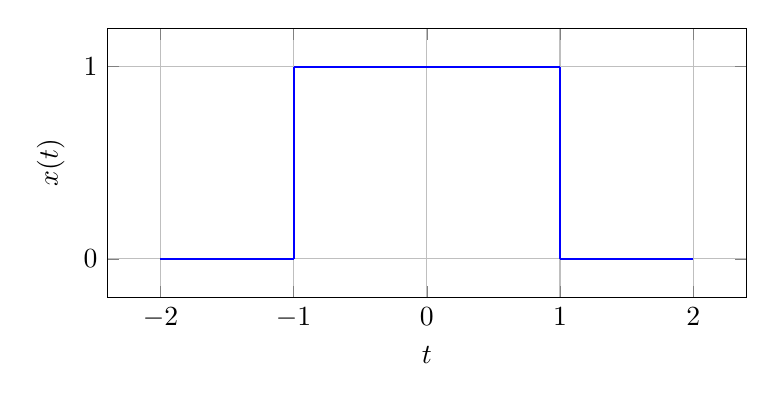
\begin{tikzpicture}
        \begin{axis} [
            width=0.8\textwidth,
            height=5cm,
            axis lines=box, % Rahmen um den Plot
            xlabel={$t$},
            ylabel={$x(t)$},
            domain=-2:2,
            samples=200,
            xtick={-2,-1,0,1,2},
            ytick={0,1},
            ymin=-0.2, ymax=1.2,
            grid=both,
        ]
        % Null-Linie links
        \addplot[blue, thick, samples=2, domain=-2:-1] {0};
        % Rechteck oben
        \addplot[blue, thick, samples=2, domain=-1:1] {1};
        % Null-Linie rechts
        \addplot[blue, thick, samples=2, domain=1:2] {0};
        % Vertikale Linie bei t=-1
        \addplot[blue, thick, samples=2, domain=0:1] ({-1},{x});
        % Vertikale Linie bei t=1
        \addplot[blue, thick, samples=2, domain=0:1] ({1},{x});
        \end{axis}
    \end{tikzpicture}
    \caption{Verlauf der Rechteckfunktion $x(t)$ mit Amplitude 1 im Intervall $-1 < t < 1$}
    \label{fig:rechteck}
\end{figure}

Die Rechteckfunktion $x(t)$ ist gegeben durch:
\[
x(t) = \begin{cases}
    1 & \text{für } -1 < t < 1 \\
    0 & \text{sonst}
    \end{cases}
\]
    
Die Fourier-Transformierte einer Rechteckfunktion der Breite $2T$ und Höhe $1$ ist gegeben durch die normierte $\mathrm{sinc}$-Funktion:
\[
\mathcal{F}\{x(t)\} = 2T \cdot \mathrm{sinc}(T\omega) = 2T \cdot \frac{\sin(T\omega)}{T\omega}
\]
Der Verlauf der Fourier-Transformierten ist in folgender Abbildung dargestellt:

\begin{figure}[h]
\centering
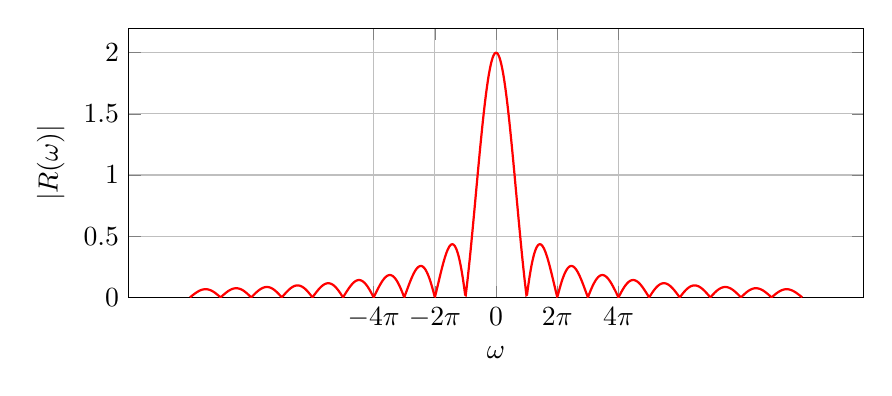
\begin{tikzpicture}
\begin{axis}[
    width=0.9\textwidth,
    height=5cm,
    xlabel={$\omega$},
    ylabel={$|R(\omega)|$},
    domain=-10*pi:10*pi,
    samples=1000,
    ymin=0, ymax=2.2,
    xtick={-12.56, -6.28, 0, 6.28, 12.56},
    xticklabels={$-4\pi$, $-2\pi$, $0$, $2\pi$, $4\pi$},
    grid=major,
]
\addplot[red, thick] {2*abs(sin(deg(x))/x)};
\end{axis}
\end{tikzpicture}
\caption{Betragsspektrum eines Rechteckpulses der Breite $T = 2$}
\label{fig:fourier_rechteck}
\end{figure}

Die Rechteckfunktion ist in der digitalen Signalverarbeitung von Relevanz, da diese eine Basis für die Änderung des Signalpegels darstellt. Durch die Idealisierung lässt sich der High-Pegel (1) und Low-Pegel (0) des Signals gut darstellen. In der Praxis wird die Rechteckfunktion jedoch durch eine $\mathrm{sinc}$-Funktion approximiert, um Übertragungsfehler zu minimieren.

\subsection{Betrag und zeitlicher Verlauf von Sinusfunktion}
Der Sinus ist eine wichtige Funktion in der Signalverarbeitung.
Er beschreibt eine harmonische Schwingung und ist in der Fourier-Analyse von Bedeutung. Sein Verlauf ist in der Abbildung \ref{fig:sinus} dargestellt.
Die Sinusfunktion $x(t) = \sin(t)$ hat eine Periode von $2\pi$ und schwingt zwischen -1 und 1. Sie ist punktsymmetrisch um den Koordinatenursprung, was bedeutet, dass $x(-t) = -x(t)$ gilt. Dies ist eine Eigenschaft der ungeraden Funktion.

\begin{figure}[H]
\centering
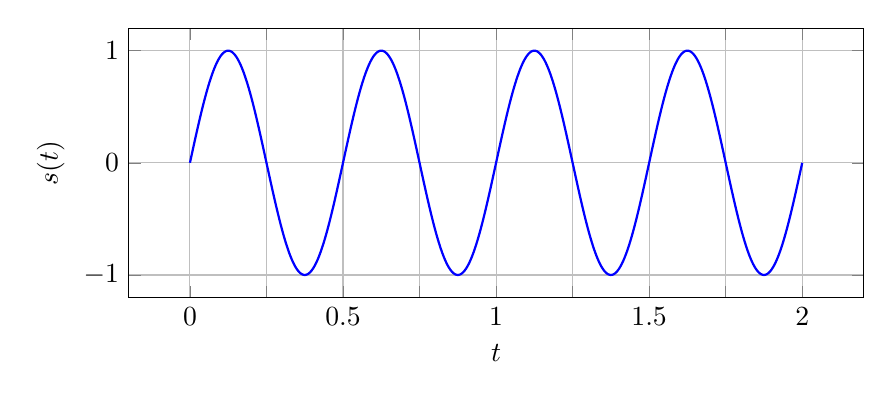
\begin{tikzpicture}
\begin{axis}[
    width=0.9\textwidth,
    height=5cm,
    xlabel={$t$},
    ylabel={$s(t)$},
    domain=0:2,
    samples=500,
    grid=major,
    xtick={0, 0.25, 0.5, 0.75, 1, 1.25, 1.5, 1.75, 2},
    xticklabels={$0$, , $0.5$, , $1$, , $1.5$, , $2$},
    ymin=-1.2, ymax=1.2,
    declare function={
        omegaNull = 4*pi;
    },
]
\addplot[blue, thick] {sin(deg(omegaNull * x))};
\end{axis}
\end{tikzpicture}
\caption{Zeitverlauf des Sinussignals $s(t) = \sin(\omega_0 t)$ mit $\omega_0 = 4\pi$}
\end{figure}



Die Fourier-Transformierte der Sinusfunktion $x(t) = \sin(t)$ ist gegeben durch:
\[
\mathcal{F}\{\sin(\omega_0 t)\} = \pi j \left[ \delta(\omega + \omega_0) - \delta(\omega - \omega_0) \right]
\]
Für $\omega_0 = 1$ ergibt sich:
\[
\mathcal{F}\{\sin(t)\} = \pi j \left[ \delta(\omega + 1) - \delta(\omega - 1) \right]
\]
Der Betrag der Fourier-Transformierten besteht also aus zwei Dirac-Impulsen bei $\omega = \pm 1$.

Die graphische Darstellung der Fourier-Transformierten der Sinusfunktion ist in Abbildung \ref{fig:fourier_sinus_komplex} zu sehen.
\begin{figure}[H]
\centering
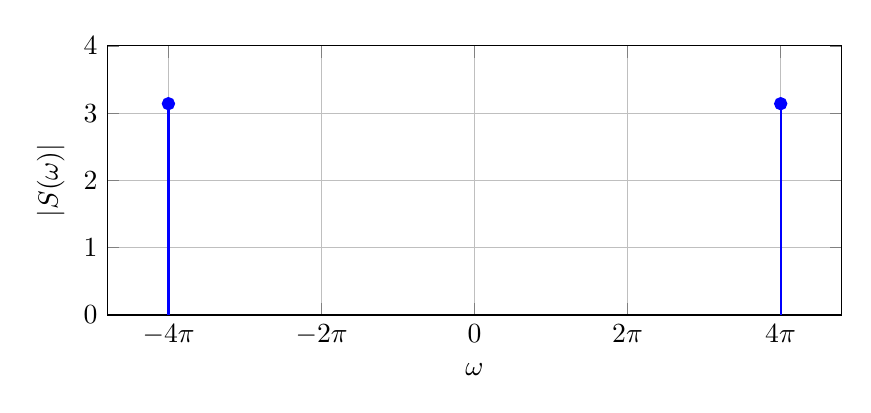
\begin{tikzpicture}
\begin{axis}[
    width=0.9\textwidth,
    height=5cm,
    xlabel={$\omega$},
    ylabel={$|S(\omega)|$},
    domain=-15:15,
    samples=1000,
    ymin=0, ymax=4,
    xtick={-12.56, -6.28, 0, 6.28, 12.56},
    xticklabels={$-4\pi$, $-2\pi$, $0$, $2\pi$, $4\pi$},
    grid=major,
]
\addplot[blue, ycomb, thick, mark=*] coordinates {(-4*pi, 3.14) (4*pi, 3.14)};
\end{axis}
\end{tikzpicture}
\caption{Betragsspektrum eines Sinussignals $s(t) = \sin(\omega_0 t)$ mit $\omega_0 = 4\pi$}
\end{figure}

Die Sinusfunktion spielt eine immens wichtige Rolle in der digitalen Signalverarbeitung, da es der Grundstein der Fourier-Analyse (Fourier-Reihen und Fourier-Transformation) ist. Auch sind diese für lineare zeitinvariante Systeme (LTI) von Bedeutung. 
Der Sinus ist eine elementare periodische Funktion, seine Periodizität ist das grundlegende Konzept in vielen Signalen. Er lässt auch unter anderem komplex erscheinende Funktionen in Sinuskomponenten zerlegen und somit sie einfacher und kompakter darstellen.
Auch in der analogen Signalverarbeitung ist der Sinus von Bedeutung, da er die Basis für die Amplituden-, Frequenz- und Phasenmodulation bildet. Schließlich ist die Idealform der aus der Steckdose kommenden Netzspannung eine Sinuswelle, die in vielen Anwendungen als Referenzsignal dient. 

\subsection{Multiplikation der beiden Funktionen im Zeitbereich}
Bei einer Multiplikation der beiden Funktionen im Zeitbereich, also der Rechteckfunktion $x(t)$ und der Sinusfunktion $y(t)$, ergibt sich eine neue Funktion $z(t) =  x(t) \cdot y(t)$, die in Abbildung \ref{fig:rechteck_sinus} dargestellt ist. Diese Funktion ist das Ergebnis der Punkt-für-Punkt-Multiplikation der beiden Funktionen.
% \begin{figure}[H]
%     \centering
%     \begin{tikzpicture}
%         \begin{axis}[
%             width=0.8\textwidth,
%             height=5cm,
%             axis lines=middle,
%             xlabel={$t$},
%             ylabel={$z(t)$},
%             domain=-2:2,
%             samples=200,
%             xtick={-2,-1,0,1,2},
%             ytick={-1,0,1},
%             ymin=-1.2, ymax=1.2,
%             grid=both,
%         ]
%         % Rechteckfunktion
%         \addplot[blue, thick, samples=2, domain=-2:-1] {0};
%         \addplot[blue, thick, samples=2, domain=-1:1] {1};
%         \addplot[blue, thick, samples=2, domain=1:2] {0};
%         % Sinusfunktion
%         \addplot[red, thick] {sin(deg(x))};
%         % Multiplikation der beiden Funktionen
%         \addplot[green, thick] {sin(deg(x)) * (x >= -1 && x <= 1)};
%         \end{axis}
%     \end{tikzpicture}
%     \caption{Multiplikation der Rechteckfunktion $x(t)$ und der Sinusfunktion $y(t)$ im Zeitbereich}
%     \label{fig:rechteck_sinus}
% \end{figure}


Die Fourier-Transformierte der Multiplikation zweier Funktionen im Zeitbereich ist gegeben durch die Faltung ihrer Fourier-Transformierten im Frequenzbereich. Das bedeutet, dass die Fourier-Transformierte von $z(t)$, also $\mathcal{F}\{z(t)\}$, das Ergebnis der Faltung der Fourier-Transformierten von $x(t)$ und $y(t)$ ist:
\[
\mathcal{F}\{z(t)\} = \mathcal{F}\{x(t)\} * \mathcal{F}\{y(t)\}
\]

Es ergibt sich also eine neue Funktion im Frequenzbereich, die die Frequenzkomponenten der beiden ursprünglichen Funktionen kombiniert.
\begin{figure}[H]
\centering
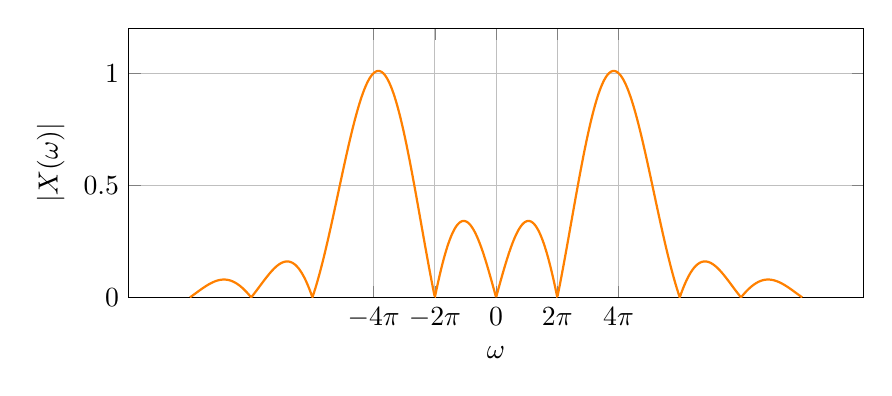
\begin{tikzpicture}
\begin{axis}[
    width=0.9\textwidth,
    height=5cm,
    xlabel={$\omega$},
    ylabel={$|X(\omega)|$},
    domain=-10*pi:10*pi,
    samples=1000,
    ymin=0, ymax=1.2,
    xtick={-12.56, -6.28, 0, 6.28, 12.56},
    xticklabels={$-4\pi$, $-2\pi$, $0$, $2\pi$, $4\pi$},
    grid=major,
]
\addplot[orange, thick] {abs(sin(deg((x-4*pi))/2)/((x-4*pi)/2) - sin(deg((x+4*pi))/2)/((x+4*pi)/2))};
\end{axis}
\end{tikzpicture}
\caption{Betragsspektrum der Fourier-Transformierten $\mathcal{F}\{z(t)\}$}
\label{fig:fourier_rechteck_sinus}
\end{figure}

\section{Zusammenhang von Datenrate und Bandbreite}
blabla
\clearpage


\chapter{HF-Simulation}
\section{Inbetriebnahme von Keysight Advanced Design System (ADS)}
\subsection{Installation von ADS}
Die Software \ac{ADS} dient zur Simulation von Schaltungen verschiedener Komplexitätsgrade. 
In diesem Versuch wird die Software verwendet, um eine Hochfrequenzschaltung zu simulieren und zu analysieren. 
Die Software bietet eine Vielzahl von Funktionen, darunter die Möglichkeit, Schaltungen zu entwerfen, S-Parameter zu simulieren und verschiedene Analysewerkzeuge zu verwenden.

\subsection{Erstellen eines neuen Projekts}
Die Software ist auf den Rechnern im Labor bereits installiert gewesen. 
Nach dem Start der Software wird ein neues Projekt aus den bereits zur Verfügung stehenden Workspaces erstellt. 
Diese sind auf der ILIAS-Seite des Praktikums in dem Dateiarchiv \texttt{TransmitterAmpDesign 2024.zip} hinterlegt. 
Die Datei wird entpackt und in der Software geöffnet. Außerdem werden die benötigten Bibliotheken aus dem Dateiarchiv \texttt{Infineon-RFTransistor-Keysight ADS Design Kit-SM-v02 10-EN.zip} geladen, diese stehen ebenfalls auf der ILIAS-Seite zur Verfügung.
\subsection{Vertrautmachen mit der Benutzeroberfläche}
Schließlich werden die Tutorials 1 und 2 von \ac{ADS} durchgearbeitet, um sich mit der Benutzeroberfläche und den grundlegenden Funktionen der Software vertraut zu machen.
Am Anfang der Schaltungsanalyse wird das Schema \texttt{TX\_Amp.dds} geöffnet.

\section{Analyse des Datenblattes zu Transistor BFR181W}
Um die Schaltung zu simulieren, wird der Transistor BFR181W verwendet. Um die genauen Parameter des Transistors zu kennen, wird das Datenblatt des Transistors analysiert.
Dieses steht auch auf der ILIAS-Seite des Praktikums zur Verfügung.

Die Tabelle \enquote{Maximum Ratings at $T_\mathrm{A}=25\,^\circ\mathrm{C}$, unless otherwise specified} unten links auf Seite 1 des Dokuments zeigt, dass der maximal zulässige Kollektorstrom $I_{C,\mathrm{max}}$ 20\,mA beträgt.
\section{DC-Simulation}
Im folgendem wird eine DC-Simulation der später aufzubauenden Schaltung durchgeführt. 
Außerdem werden die Arbeitspunkte optimal durch die Anpassung der Widerstandswerte eingestellt.
Die DC-Simulation wird in \ac{ADS} durchgeführt, um die DC-Pegel der Schaltung zu überprüfen.

Folgende Spannungswerte werden angenommen:
\begin{itemize}
    \item $U_{CC} = 4.8\,\mathrm{V}$
    \item $U_{BE} = 0.77\,\mathrm{V}$
\end{itemize}

Zuerst wird der Kollektorwiderstand $R_5$ passend gewählt, sodass der Kollektorstrom $I_C$ auf $75\,\%$ des maximal zulässigen Kollektorstroms $I_{C,\mathrm{max}}$ gesetzt wird. 
Dies geschieht, indem der Widerstandswert $R_5$ so gewählt wird, dass der Kollektorstrom $I_C$ 15\,mA beträgt.
Der Widerstandswert $R_5$ wird mit folgender Formel berechnet:
\begin{equation}
    R_5 = \frac{U_{CC} - U_{CE}}{I_C} = \frac{4.8\,\mathrm{V} - 0.77\,\mathrm{V}}{15\,\mathrm{mA}} = 274.67\,\Omega
\end{equation}

Bei der Verwendung der E12-Reihe wird eine Faustregel verwendet, nach der man die Widerstandswerte auf die nächstgelegene E12-Reihe aufrundet. 
Somit beträgt der Widerstandswert von $R_5$ 330\,\(\Omega\). Dadurch wird der in den Kollektor eingehende Strom beschränkt, was eine Überlastung des Transistors im Dauerbetrieb vorbeugt.
\section{S-Parameter-Simulation}

blabla
\clearpage


\chapter{Technische Umsetzung}

\section{Platinen Aufbau}
Die Platine ist mit mehreren Bauteilen ausgestattet, die bis auf drei selbstdimensionierten Widerständen
bereits vollständig bestückt ist. \\
% Auf dem Schaltplan  (R Widerstand, C Kondensator, J Stecker/Relais)% 
\\
Zur Erkärung von Abbildung 4.1 hier eine kurze Information zu den wichtigsten Abkürzungen:
\begin{itemize}
    \item R: Widerstand
    \item C: Kondensator
    \item J: Stecker/Relais

    
\end{itemize}
%mache wir die Bilder 1-3 auch rein?
Die wichtigsten Bauteile sind:
%Frage: Generell wichtig oder nur für das was wir bei diesem Versuch machen? USB Buchse hier irrelevant....
\begin{itemize}
    \item J1: Anschluss an den FieldFox (Ausgangssignal)
    \item J40: Verbindung zu Oszillator (Taktquelle für die Schaltung) und Anschluss an den FiedFox (Eingangssignal)
    \item R47-49: Widerständ zur Arbeitspunkteinstellung
    \item Oszillator (XLL536C50.000000X): HF-Taktsignal
    \item Transistor (BFR181W) 
    \item Operationsverstärker (U20-LMV651MG/NOPB; U21-NCX2200GW,125)
    \item USB UART IC (FT232RL)
\end{itemize}

\begin{figure}[h]
    \centering
    \includegraphics[width=1.0\textwidth]{Pictures/Bestückungsplan.jpg}
    \caption{Bestückungsplan}
\end{figure}



\section{Bestückung PCB}
Die in Kapitel 3 bestimmten Widerstände werden nun im Rahmen der praktischen Umsetzung der Schaltung auf die 
bereits vorbereitete Platine angebracht. Auf dem Bestückungsplan entspricht hier R47 R3 mit 1000 Ohm, R48 R4 mit 
4700 Ohm und R49 R5 mit 330 Ohm. Bei dem Löten der drei Widerständen wird auf eine saubere und präzise Löttechnik
geachtet um die gewollte elektrische, mechanische und HF-technische Funktion der Schaltung zu garantieren. 
\begin{figure}[h]
    \centering
    \includegraphics[width=0.54
    \textwidth]{Pictures/Platinebestückt.jpg}
    \caption{Bestückungsplan}
\end{figure}


\section{DC-Pegel Verifizieren}
Nach dem Bestücken der Platine wird die Funktionalität der Schaltung überprüft. Hierzu wird eine Versorgungsspannung von 
4.8V angelegt um den Gleichspannungspegel an den relevanten Punkten der Schaltung zu überprüfen. Die abfallenden 
Spannungen werden mit einem Oszilloskop gemessen. Releavnt sind die Spannungsabfälle über R47, R48 und R49. Diese gemessenen
Spannungen werden mit den idealen Werten 
der Simulation verglichen. 

\section{SOLT-Kalibrierung}
Das Ziel der SOLT-Kalibrierung (Short, Open, Load, Through) ist die elemenierung
von systematischen Messfehlern. Die durch die Messausrüstung(Kabel,Adapter, etc.)
selbst entstehen und die Messung verfälschen.
Durch Messen von diesen Fehlern lässt sich die Messung korrigieren.
Dafür werden vier verschiedene Kalibrierstandards benötigt:
\begin{itemize}
    \item Short (Kurzschluss): Ein Kurzschluss-Standard wird an den Messport des VNAs angeschlossen. Da ein idealer Kurzschluss alle Leistung reflektiert und eine Phasenverschiebung von 180 Grad verursacht, misst der VNA diese Referenz. Abweichungen vom Ideal werden erfasst. 
    \item Open (Leerlauf): Ein Leerlauf-Standard wird angeschlossen. Ein idealer Leerlauf reflektiert ebenfalls die gesamte Leistung, jedoch mit einer Phasenverschiebung von 0 Grad. Auch hier werden Abweichungen aufgezeichnet.
    \item Load (Abschluss/Last): Ein Präzisions-Abschlusswiderstand (meist 50 Ohm) wird angeschlossen. Ein idealer Abschlusswiderstand absorbiert die gesamte Leistung ohne Reflexion. Dies dient dazu, die Leistungsanpassung des Systems zu kalibrieren.
    \item Through (Durchgang): Bei einer 2-Port-Messung wird ein direkter Durchgang (ein kurzes, bekanntes Kabel oder ein Adapter) zwischen den beiden Messports des VNAs angeschlossen. Dies ermöglicht die Kalibrierung der Übertragungseigenschaften zwischen den Ports und die Korrektur von Phasen- und Amplitudenfehlern des Übertragungspfades.
\end{itemize}
%(erklärung warums tut)
\section{Vergleich zur Simulation}
Ergebnisse SImulation Farhad vergleichen mit Notizen Farhad.
\clearpage


\chapter{Ergebnisse}


\section{Tabellen und Diagramme}
bla bla
\clearpage

\chapter{Diskussion}
\section{Vergleich von Theorie und Praxis}
\section{Erklärung von Abweichungen}
bla bla
\clearpage

\chapter{Fazit}

\section{Zusammenfassung der wichtigsten Erkenntnisse}
\section{Reflexion und mögliche Verbesserungen}
\section{Eigene Reflexion}
\subsection{Erik}
\subsection{Farhad}
\subsection{Lukas}
bla bla
\clearpage

\chapter{Literaturverzeichnis}

\begin{thebibliography}{1}
\bibitem{microstrip_filters}
Hong, J.-S.; Lancaster, M. J.: \emph{Microstrip Filters for RF/Microwave Applications}, 2., überarbeitere Auflage. Hoboken, NJ: Wiley-Blackwell, 2011. ISBN 978-0-470-40877-3.

\bibitem{SchaltplanPCBV4}
Simon Haussmann: \emph{Schaltplan\_PCB\_V4}, 15. April 2024. In: Institut für Robuste Leistungshalbleitersysteme, Universität Stuttgart. Online verfügbar unter: \url{https://ilias3.uni-stuttgart.de/ilias.php?baseClass=ilrepositorygui&cmdNode=z5:o1&cmdClass=ilObjFileGUI&cmd=sendfile&ref_id=4067155} (zugegriffen am 19.05.2025)


\bibitem{Microstip}
Autor unbekannt: \emph{Microstrip}. In: Microwave101 Online verfügbar unter:\url{https://www.microwaves101.com/encyclopedias/microstrip} (zugegriffen am 02.06.2025)


\bibitem{RF Band Pass Filter}
Eyal Cohen: \emph{RF Band Pass Filter}. In: Medivague : \url{https://medivague.com/bpf-coupled-line-theory/} (zugegriffen am 01.06.2025)

\bibitem{Parallel Coupled Lines}
Autor unbekannt: \emph{Parallel Coupled Lines}. In: Libre Texts Engineering : \url{%https://eng.libretexts.org/Bookshelves/Electrical_Engineering/Electronics/Microwave_and_RF_Design_IV%3A_Modules_(Steer)/03%3A_Parallel_Coupled-Line_Filters/3.02%3A_Parallel_Coupled_Lines} (zugegriffen am 01.06.2025)


\bibitem{Kalibrierung}
Dr.  Latzel, Georg: \emph{SOLT Kalibrierung}. In: dl6gl Amateurfunk : \url{https://dl6gl.de/vnwa-kalibrierung.html} (zugegriffen am 20.05.2025) Zum Kopieren






\end{thebibliography}

%https://medivague.com/bpf-coupled-line-theory/
%https://eng.libretexts.org/Bookshelves/Electrical_Engineering/Electronics/Microwave_and_RF_Design_IV%3A_Modules_(Steer)/03%3A_Parallel_Coupled-Line_Filters/3.02%3A_Parallel_Coupled_Lines
\clearpage








\end{document}  % The End
%% ----------------------------------------------------------------